\subsection{Results}
\label{sec:eval}
%
\niparagraph{Throughput.}
%
Figure~\ref{fig:eval-end-to-end} reports the throughput comparison results between the three baselines and \neupims. 
%
The GPU-only and NPU-only baseline systems show marginal differences since they both execute end-to-end decoder block operations without PIM, including bandwidth-bound multi-head attention.
%
Simply integrating PIM with the NPU, i.e., NPU+PIM already offers, on average 1.5$\times$ throughput improvement compared to the NPU-only baseline because the bandwidth-bound GEMV operations in MHA are all offloaded to the PIM.
%
However, \neupims consistently surpasses the NPU+PIM baseline, and offers \emph{additional} throughput improvements over the NPU+PIM baseline across all the models and datasets, ranging from 13\% to 3$\times$.
%
These trends are observed consistently for both datasets, with larger gains observed for ShareGPT, given its longer input/output sequences, offering increased acceleration opportunities for PIMs.
%
Furthermore, as the batch size increases from 64 to 512, the throughput gains exhibit substantial growth. 
%
This is because the \neupims system effectively shifts the bottleneck from bandwidth to compute towards the NPU, thus allowing \neupims to extract higher performance from batched computation as the batch size grows. 
%
Note that \neupims achieves significant throughput improvements using the same memory capacity, which demonstrates its cost-effectiveness, especially in a datacenter-scale inference serving scenario where larger batch sizes are advantageous.  

%
\begin{table}[]
\centering
\caption{Average resource utilization of NPU/PIM compute resource and memory bandwidth utilization.}
\label{tab:util}
\small
\vspace{-2ex}
\begin{tabular}{c|c|c|c}
\hline
          & \textbf{NPU-only}          & \textbf{NPU+PIM}          & \textbf{\textsc{NeuPIMS}}         \\ \hline
NPU       & 12.3\%         & 28.0\%             & \textbf{64.9}\%   \\
PIM       & -               & 17.0\%             & \textbf{26.4\%}   \\
Bandwidth & 67.6\%         & 27.4\%             & \textbf{85.4\%}   \\
\hline
\end{tabular}
\end{table}
% sharegpt 30B batchsize 256
% layer 48 / 2
%
\niparagraph{Utilization.}
%
The main source of large throughput gain is the improved resource utilization across the board. 
%
Table~\ref{tab:util} compares the average utilization for three major resources in the baselines and \neupims, when using GPT3-30B, the batch size of 256, and the ShareGPT dataset.  
%
As NPU+PIM offloads the bandwidth-bound MHA operations to PIM, it increases NPU utilization by 28.0\%.
%
However, NPU+PIM still suffers from temporal blocking due to the GEMM-GEMV dependencies in LLM inferencing. 
%
\neupims overcomes this limitation, achieving 64.9\% and 26.4\% utilization on NPU and PIM, respectively, through the concurrent NPU+PIM execution capability.
% 
We observe similar trends from the other system configurations, which demonstrate the effectiveness of the proposed technique in enabling concurrent NPU+PIM execution by \neupims.

%
\begin{figure}[t]
        \centering
        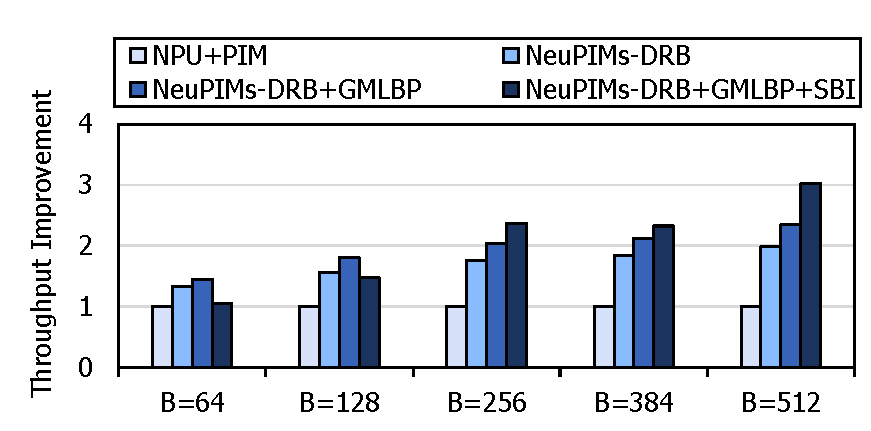
\includegraphics[width=0.95\linewidth]{figure/batch-throughput.pdf}
        \vspace{-2ex}
        \caption{We use the GPT3-7B model and ShareGPT dataset for this experiment. DRB: Dual Row Buffers; GMLBP: Greedy Min-Load Bin Packing algorithm; SBI: Sub-Batch Interleaving.}
        \vspace{-2ex}
        \label{fig:batch-size-sensitivity}
\end{figure}
%


\niparagraph{Ablation study.}
%
Using NPU+PIM as the baseline, we augment the proposed three techniques and observe the performance behaviors, shown in Figure~\ref{fig:batch-size-sensitivity}. 
%
For all batch sizes, the dual row buffers offer 69.7\% throughput improvement on average, which has the largest impact on the performance as it enables concurrent NPU+PIM execution without significant overhead. 
%
For the channel loading balancing, our greedy min-load bin packing algorithm also always offers performance benefits by evenly distributing the requests to the available channels.
%
In contrast to the previous two techniques, the sub-batch interleaving technique does not always yield gains. 
%
For small batch sizes, partitioning the batch into two may cause underutilization in a NPU systolic array, leading to inefficiency, and the penalty from pipelining could outweigh the benefits.
%
However, when the batch size is equal to or larger than 256, \neupims achieve the highest throughput, suggesting that batched inference with a large batch size is preferable for the \neupims-based system.

%
\begin{figure}[]
        \centering
        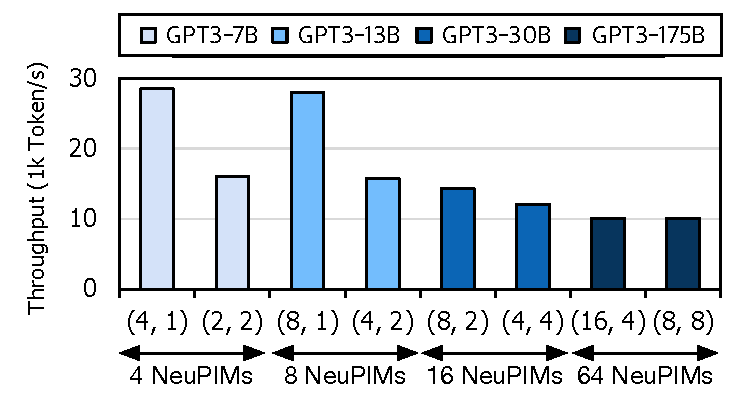
\includegraphics[width=0.95\linewidth]{figure/tp-pp.pdf}
        \vspace{-1ex}
        \caption{Throughput of multi-\neupims system as the parallelization schemes change. We employ four combinations of tensor parallelism (TP) and pipeline parallelism (PP), represented as (TP, PP).} 
        \vspace{-2ex}
        \label{fig:system-scale-sensitivity}
\end{figure}

\niparagraph{Implication of parallelization schemes.}
%
As the LLM size increases, the \neupims system must scale the number of devices to harness tensor and pipeline parallelisms.
%
Figure~\ref{fig:system-scale-sensitivity} analyzes the implications of such parallelization schemes on the system throughput. 
%
For the experiment, we fix the total number of requests to 256, while the batch size per device varies depending on the parallelization scheme. 
%
The results highlight the preference for exploiting tensor parallelism over the pipeline counterpart, as it maintains a large batch size, resulting in better efficiency at the NPU. 
%
We observe this trend consistently for all model variants, while the overall throughput decreases since the per-device batch size becomes small, due to low NPU utilization. 
%



